\documentclass[8pt, a4paper, onesided]{article}
\usepackage[left=0.1in,right=0.1in,top=0.25in,bottom=0.1in,headsep=0.05in]{geometry}
\usepackage{hyperref}
\usepackage{fancyhdr}
\usepackage{listings}
\usepackage{xcolor}
\usepackage{tocloft}
\usepackage{pdflscape}
\usepackage{multicol}
\usepackage{titlesec}
\usepackage{minted}
\usepackage{amsmath}
\usepackage{graphicx}

\usemintedstyle{default}

\setlength{\columnsep}{0.4cm}
\setlength{\columnseprule}{0.1pt}
\setlength{\parskip}{-4.5mm plus 0.5mm minus 0.5mm}

\setlength{\fboxsep}{1pt}%
\setlength{\fboxrule}{0.01pt}%

\titleformat{\section}{\normalfont\fontsize{10}{15}\bfseries}{\thesection}{1em}{}
\titleformat{\subsection}{\normalfont\fontsize{10}{13}\bfseries}{\thesubsection}{0.5em}{}
%\titleformat{\subsection}{\normalfont\bfseries}{\thesubsection}{1em}{}[\vspace*{-3.75ex}]
%\titlespacing*{\subsection}
%{0pt}{-1.75ex plus 1ex minus 1ex}{-2ex plus 1ex minus 1ex}

%\renewcommand{\ttdefault}{pcr}
\renewcommand\cftsecfont{\fontsize{10}{11}\bfseries}
\renewcommand\cftsecpagefont{\fontsize{10}{11}\mdseries}
\renewcommand\cftsubsecfont{\fontsize{8}{9}\mdseries}
\renewcommand\cftsubsecpagefont{\fontsize{8}{9}\mdseries}
\renewcommand\cftsecafterpnum{\vspace{-0.5ex}}
\renewcommand\cftsubsecafterpnum{\vspace{-0.5ex}}

\renewcommand{\theFancyVerbLine}{
  \sffamily\textcolor[rgb]{1.5,0.5,0.5}{\scriptsize\arabic{FancyVerbLine}}}
  
\lstset{escapechar=\$}

\setminted{breaklines, breaksymbolleft=\space,
breakafter={,+-*;>=}, breakbefore={</}, tabsize=2, obeytabs, mathescape, frame=topline, framesep=3pt, fontsize=\fontsize{9}{9}}

\pagestyle{fancy}
\fancyhead[L]{KUET\_Effervescent Team Notebook - \today}
\fancyhead[R]{\thepage}
\fancyfoot[C]{}

\fancypagestyle{plain}
{
\fancyhead[L]{KUET\_Effervescent Team Notebook - \today}
\fancyhead[R]{\thepage}
\fancyfoot[C]{}
}

\title{\vspace{-2.5ex}KUET\_Effervescent Team Notebook}
\author{Md. Mehrab Hossain Opi, Arnob Sarker,\\Sharif Minhazul Islam}
\date{}

\graphicspath{ {./images} }

\begin{document}
\begin{landscape}
\begin{multicols*}{3}

\maketitle
\vspace{-7ex}
\tableofcontents
\pagestyle{fancy}
 
\raggedbottom
\input contents.tex
\end{multicols*}

\begin{figure}[]
    \centering
    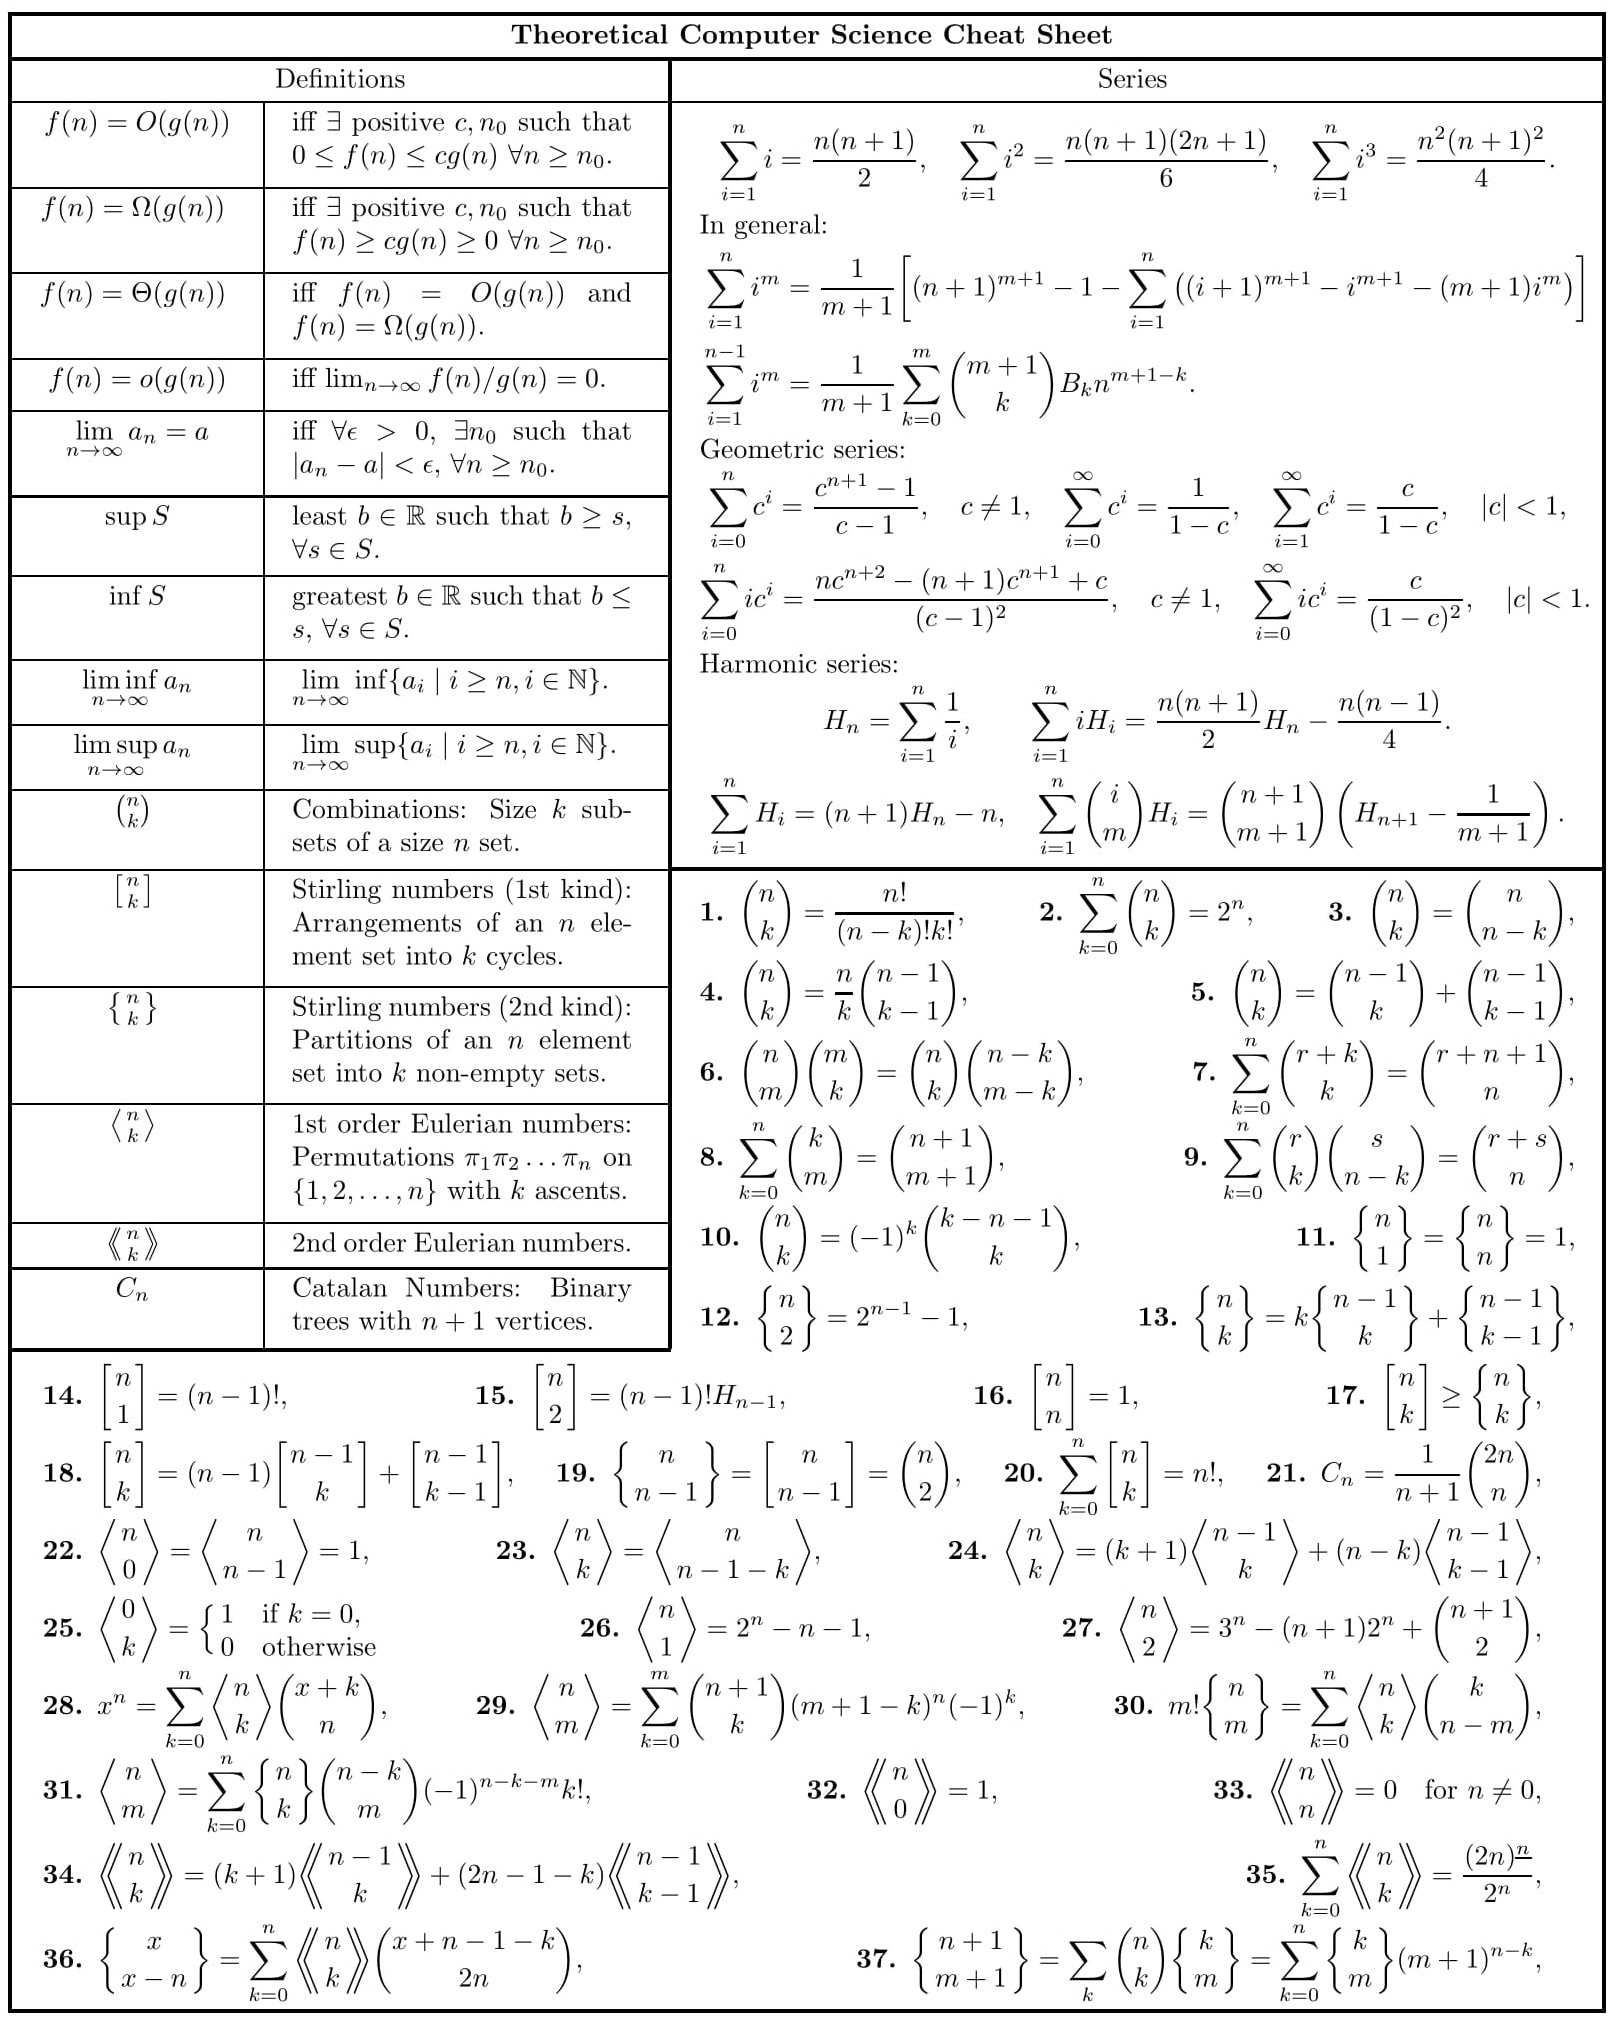
\includegraphics[width=\textheight, angle=-90]{form0}
\end{figure}
\begin{figure}[]
    \centering
    \fbox{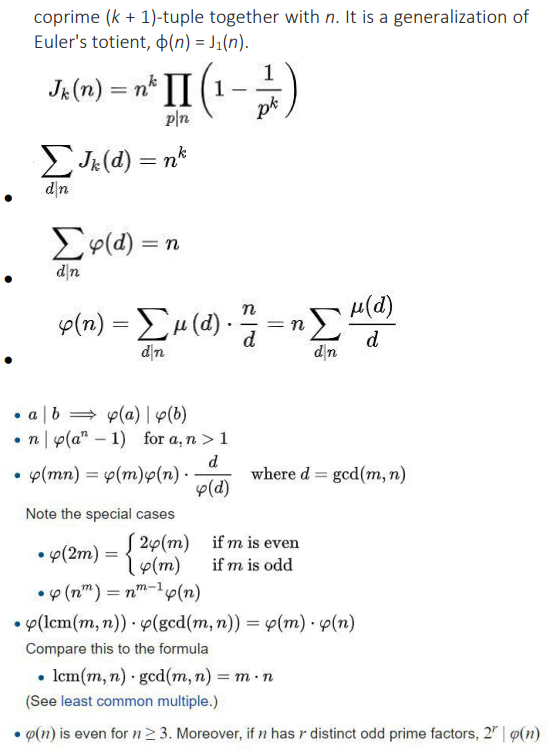
\includegraphics[height=\textwidth/2, angle=0]{1.1}}
    \fbox{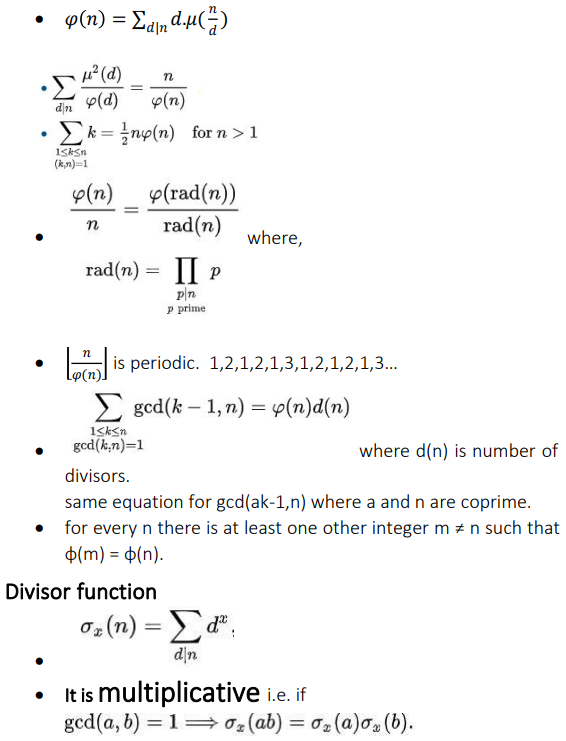
\includegraphics[height=\textwidth/2, angle=0]{1.2}}
    \fbox{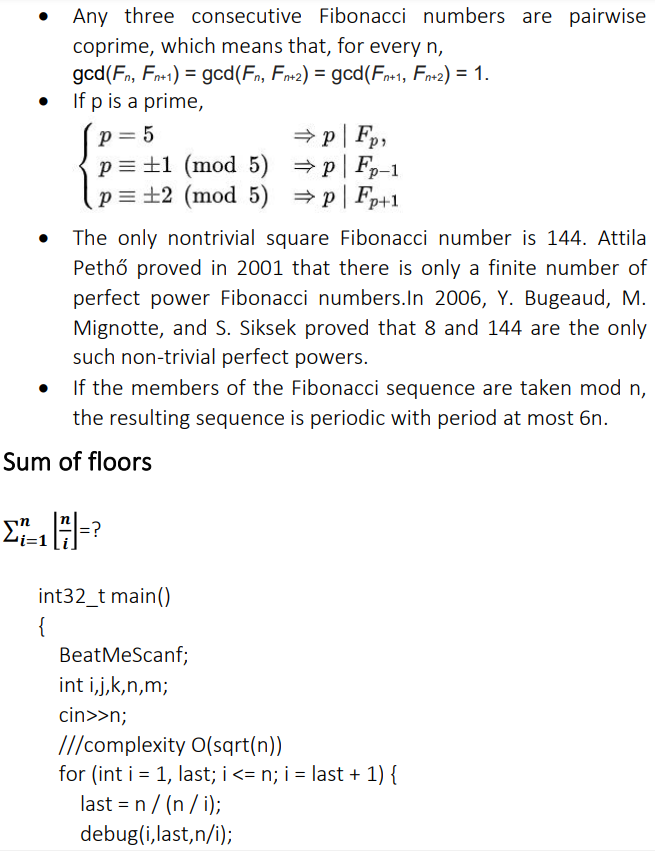
\includegraphics[height=\textwidth/2, angle=0]{2.1}}
    \fbox{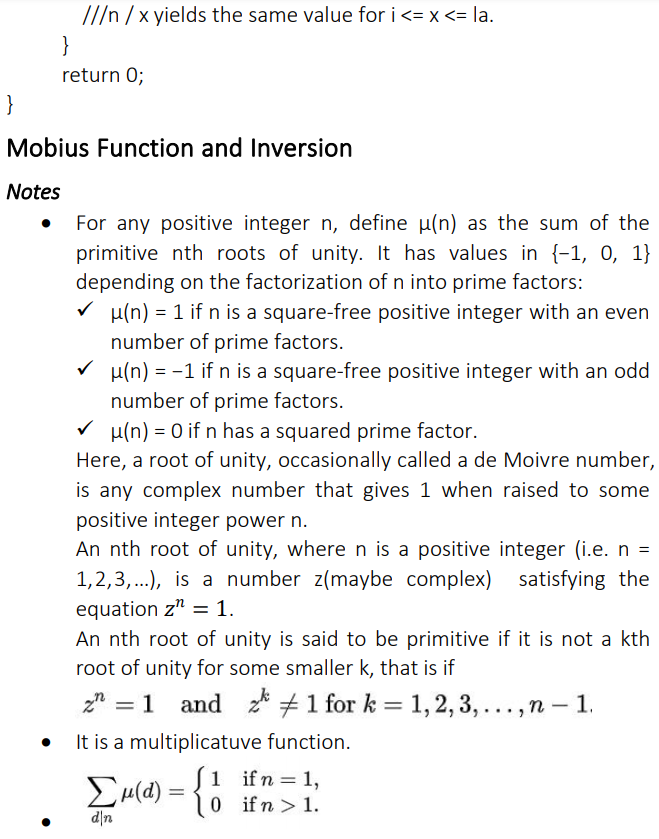
\includegraphics[height=\textwidth/2, angle=0]{2.2}}
    \fbox{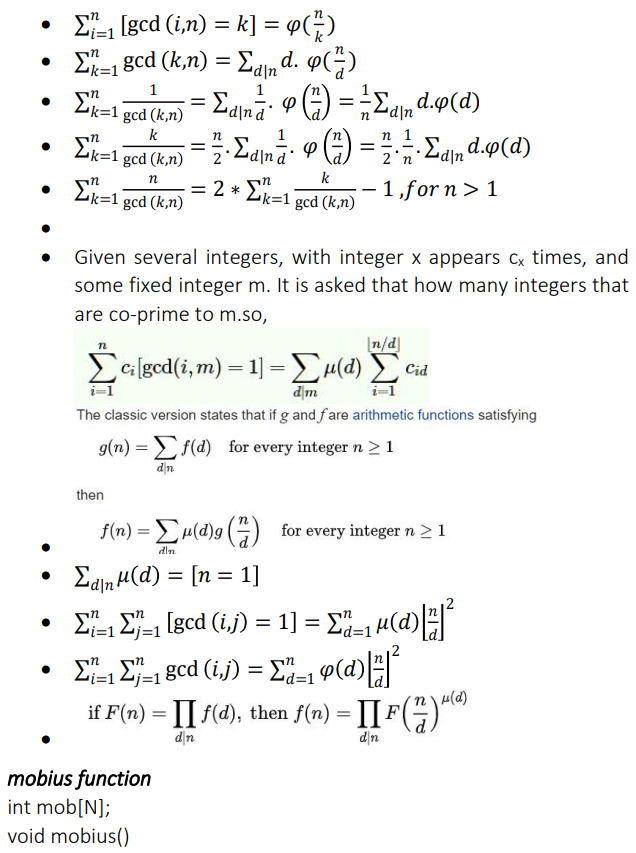
\includegraphics[height=\textwidth/2, angle=0]{3.1}}
    \fbox{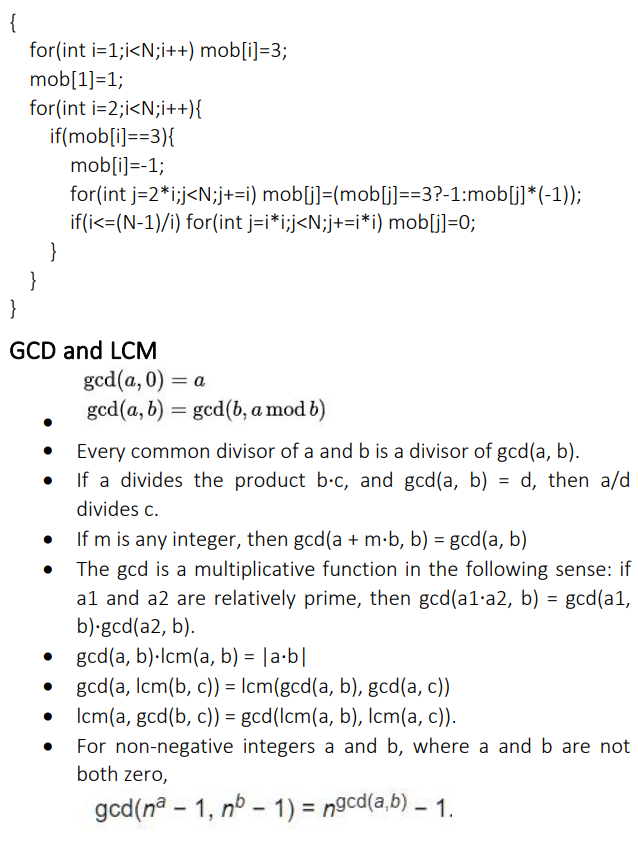
\includegraphics[height=\textwidth/2, angle=0]{3.2}}
\end{figure}
\begin{figure}[]
    \centering
    \fbox{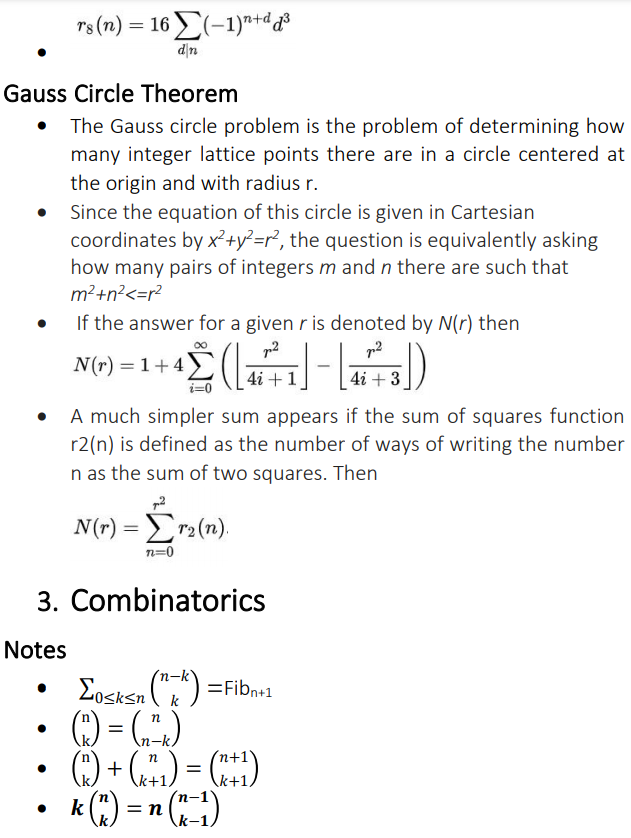
\includegraphics[height=\textwidth/2, angle=0]{4.1}}
    \fbox{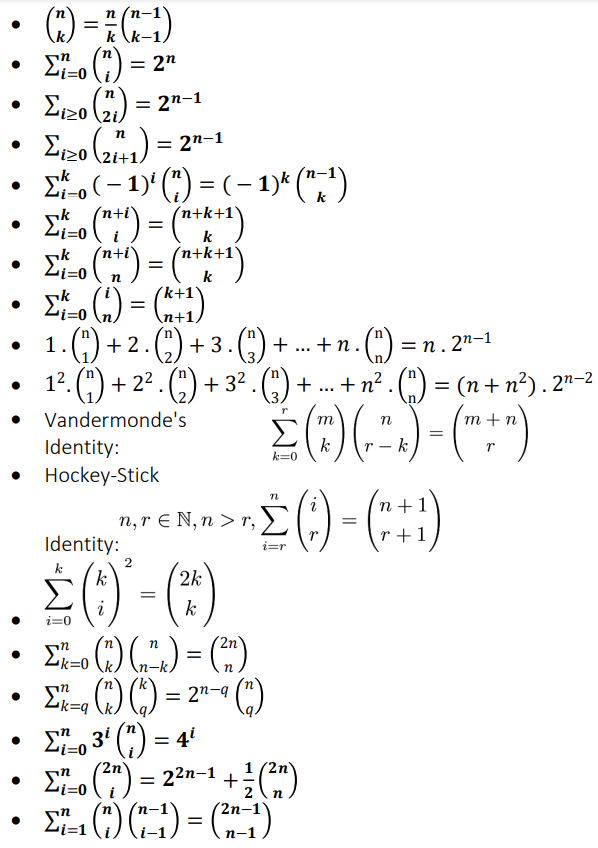
\includegraphics[height=\textwidth/2, angle=0]{4.2}}
    \fbox{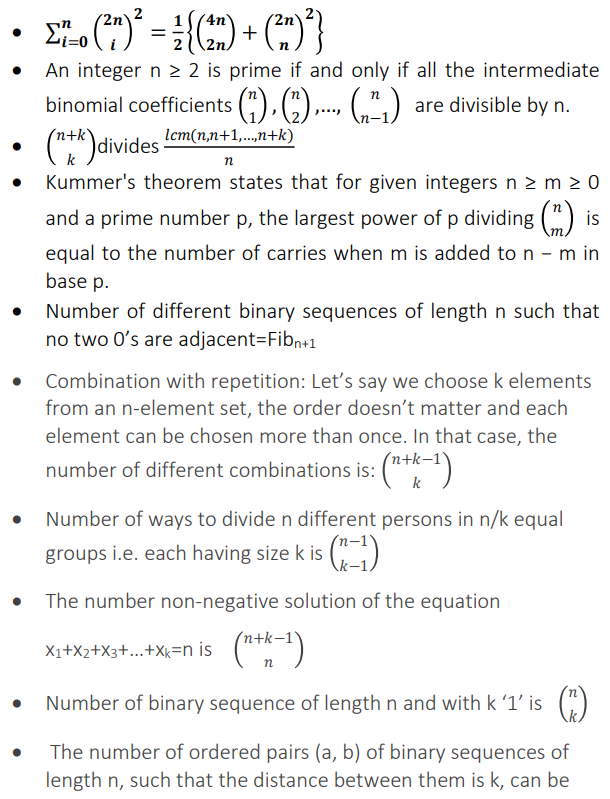
\includegraphics[height=\textwidth/2, angle=0]{5.1}}
    \fbox{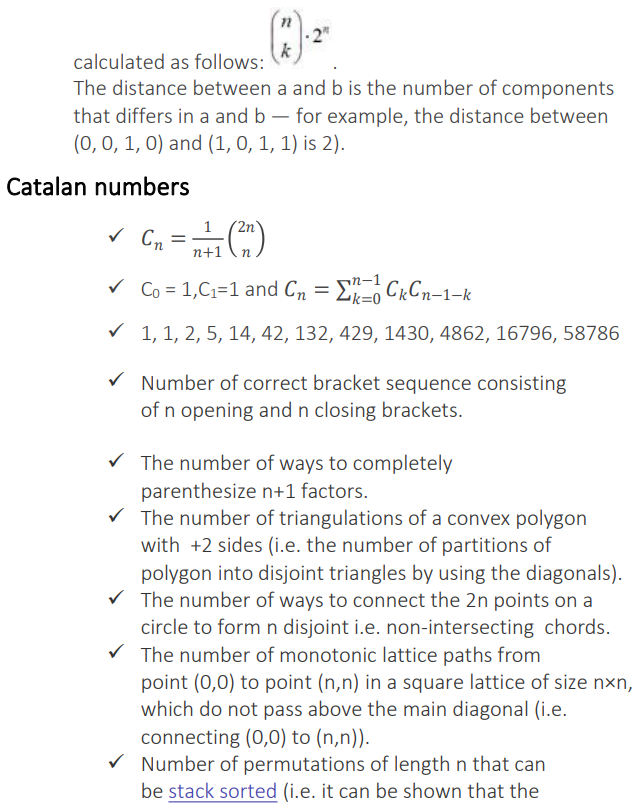
\includegraphics[height=\textwidth/2, angle=0]{5.2}}
    \fbox{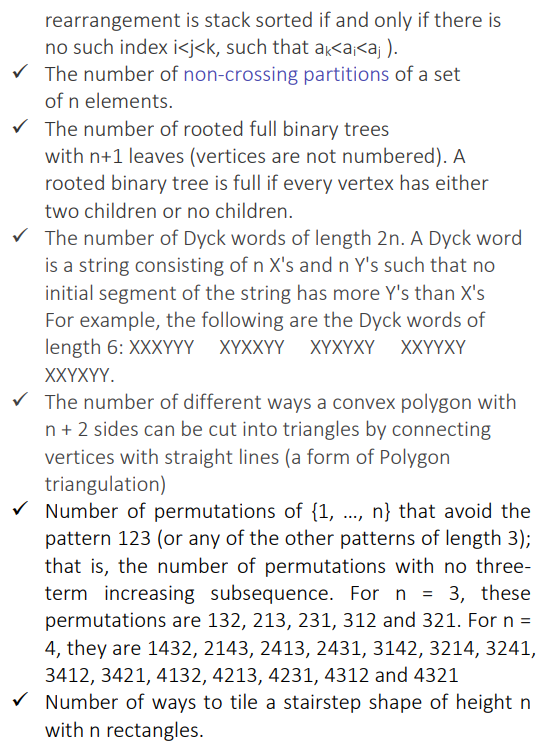
\includegraphics[height=\textwidth/2, angle=0]{6.1}}
    \fbox{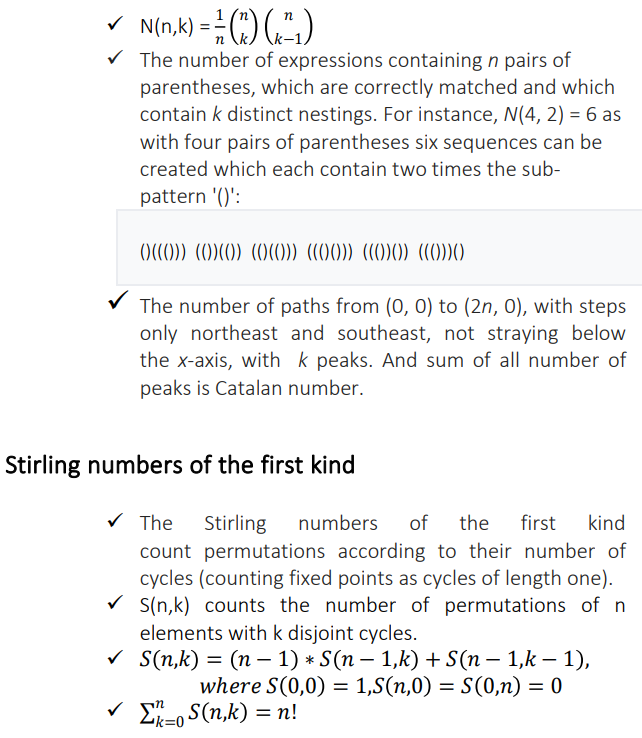
\includegraphics[height=\textwidth/2, angle=0]{6.2}}
\end{figure}
\begin{figure}[]
    \fbox{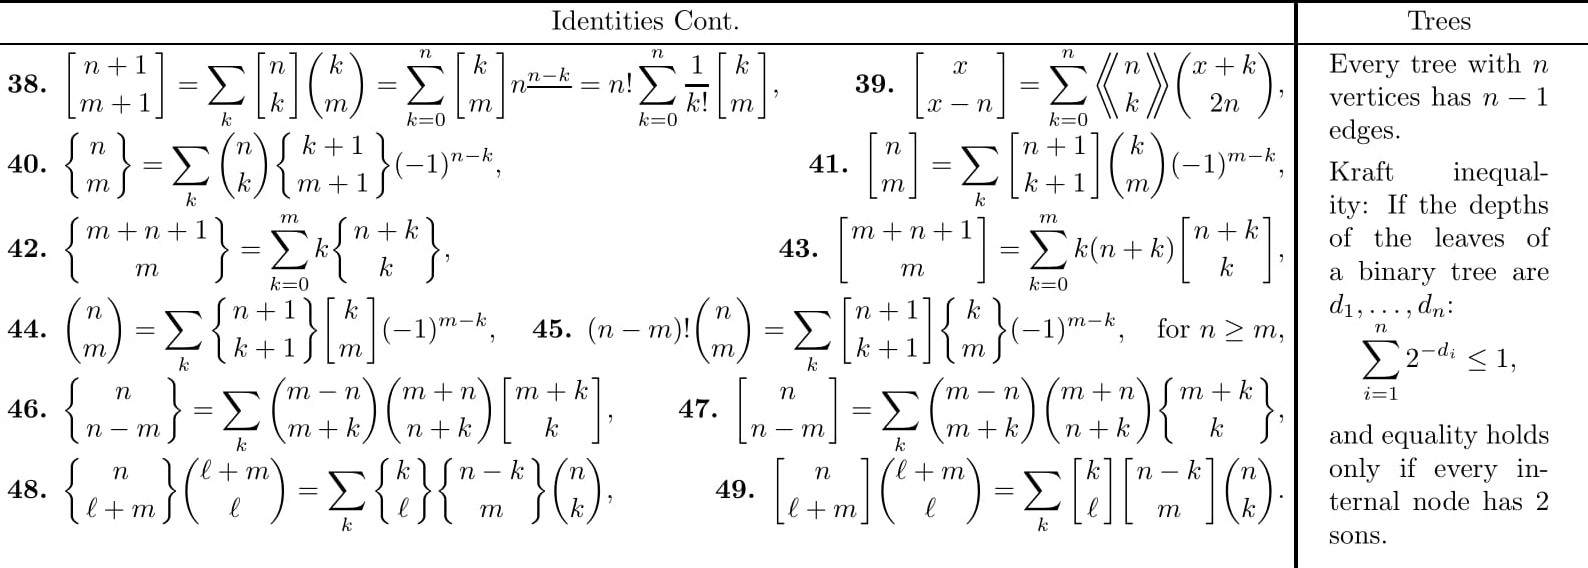
\includegraphics[height=7cm, angle=0]{14}}	
    \fbox{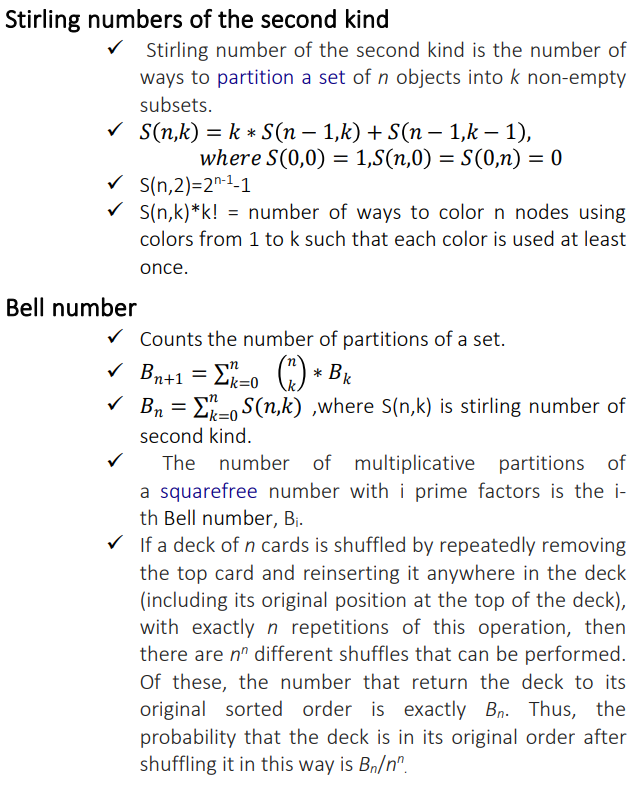
\includegraphics[height=\textwidth/2, angle=0]{7.1}}\\
    \fbox{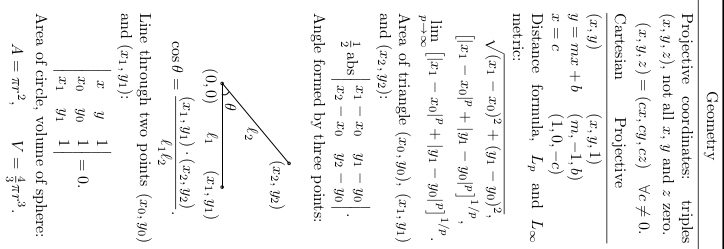
\includegraphics[height=6.75cm, angle=0]{12}}
    \fbox{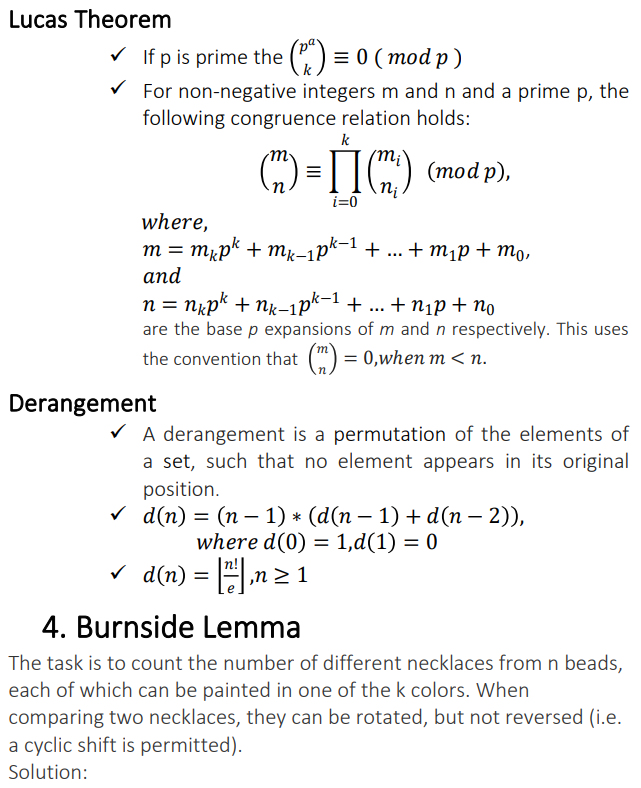
\includegraphics[height=\textwidth/2, angle=0]{7.2}}
    %\fbox{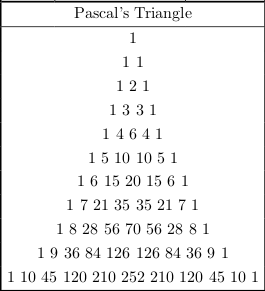
\includegraphics[height=\textwidth/2, angle=-90]{13}}
\end{figure}
\begin{figure}[]
    \fbox{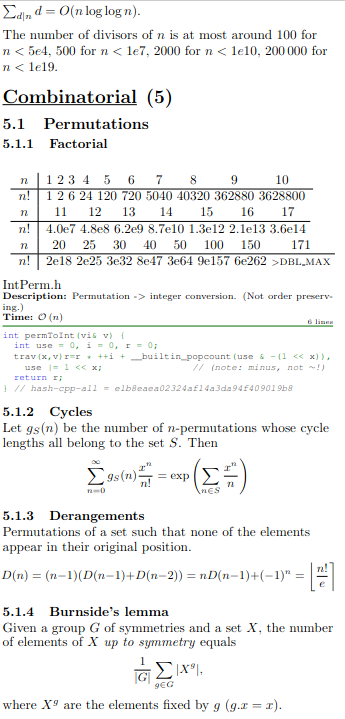
\includegraphics[height=\textwidth, angle=0]{11}}
    \fbox{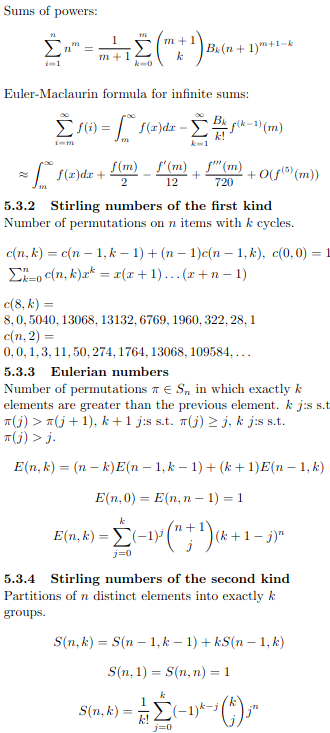
\includegraphics[height=\textwidth, angle=0]{8}}
    \fbox{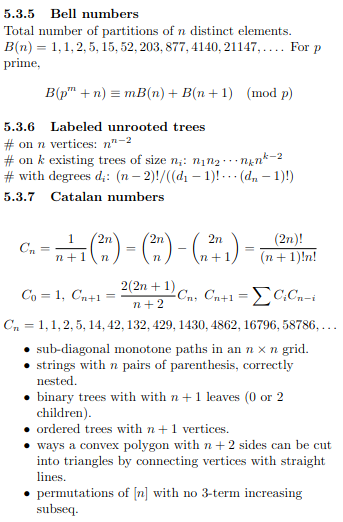
\includegraphics[width=9.25cm, angle=0]{9}}
\end{figure}
\end{landscape}
\end{document}
